\chapter{Methodology}%
\label{chapter:methodology}

\begin{introduction}
This chapter presents the non-functional requirements and the use cases of the applications. 
\end{introduction} 




\section{Applications Requirements} 


To identify the requirements of the application, I used the FURPS model. 
The non-functional requirements are listed below:

\begin{itemize}
  \item Scalability – The system should be able to support users from Europe.
  \item Reliability – The system should have a high availability of 99\% and the system also should not take longer than 4 hours to recover from a failure.
  \item Performance – The system should not take longer than 2 seconds to respond.
  \item Usability – The train of a new user should not take longer than 8 hours.
  \item Supportability – The system should be supported on the web browsers Chrome, Firefox, Microsoft Edge, and Safari.
\end{itemize}

As mentioned in Chapter II, the dealership application is structured into four key user roles: receptionist, mechanic, warehouse operator, and workshop manager.
There is a also a client aplication and an administrator.
The fuctional requirements are written below:
To manage the system it is needed an administrator to accomplish the following tasks.
- Create, change, view and remove tasks types
- Create, change, view and remove dealerships
  - Add and remove vehicle types that a dealership can operate
- Create, change, view and remove vehicle parts
- Create and view dealership employee

To interact with the client it is need a rececionist. The requirements are:
- can change betwen english and portuguese
- see number of working hours in a day 
- see the working hours of a user in a day 
- Schedule a vehicle reception date with the following information
  - vehicle registration number
  - client email
  - owner name (if applicable)
  - vehicle reception date
- create a maintenance with an expected budger, the tasks that should be performed and am expected conclusion date
- see active maintenances with the following information:
  - the name of the client
  - with the vehicle registration number
  - The entity of the vehicle if applicable
  - the creation date of the maintenance
  - evaluation date
  - expected conclusion date
  - expected budget
  - Number of hours of work expected
  - the tasks planed to be perfomerd
- The rececionist should receive a notification if there is a change in the expected budget or the expected conclusion date of the maintenance
- the rececionist should be able to confirm or reject changes of the maintenance
- the rececionist should be able to cancel the maintenance
- conclude a maintenance
- Notify when a maintenance has all planed tasks concluded 

the mechanic should be able to:
- can change betwen english and portuguese
- see the tasks needed for todays date
- pause a task, for per example, lunch hour
- continue a task
- see the following information in a maintenance task 
  - the vehicle registration number
  - type of the task
  - vehicle parts
  - description of each step to conclude a task
  - part needed to conclude the task
  - tarefas pretendidas pelo cliente
- finalize a task
- write a comment on a task before complete it 
- see the following information in an evaluation task
  - the tasks needed to do the maintenance
  - client comment
- if the dealership does not do evaluations, when finish an evaluation task, finish the maintenance with the tasks selected

the warehouse manager should do:
- can change betwen english and portuguese
- see the Inventory of the dealership with the following information for each part:
  - part name
  - part code
  - quantity available
  - location code in the warehouse
  - description
  - part category
  - price per unit
  - quantity per group
  - minimum value to generate alarm
  - maximum value
  - quantity to generate an automatic purchase requested
  - quantity in the automatic purchase request
- it should be able to edit the information of a part type, like:
  - location code in the warehouse
  - minimum value to generate alarm
  - maximum value
  - quantity to generate an automatic purchase requested
  - quantity in the automatic purchase request
- it should be able to see the movements of the quantity of each part in time 
- it can see the suppliers with the info:
  - name
  - phonenumber
  - email
  - address
  - list of parts in the contract and the start date and end date of each of them
- create a purchase with the following information:
  - motive
  - parts
  - quantity for each part
- it can see the details of all purchase like
 - the state
 - arrival date
 - total price
 - motive
 - creation date
 - parts of the purchase with:
  - the name of the part
  - quantity in stock
  - price 
  - tasks associated with this purchase
- it can register a purchase by selecting a expected arrival date in a assigned purchase
- it can register a delay on a waiting delivery purchase by selecting a new expected arrival date
- it can finalize a waiting delivery purchase by registering the parts received

The workshop manager can do:
- can change betwen english and portuguese
- see number of working hours in a day 
- see the working hours of a user in a day 
- see the tasks that doesn't have a mechanic assigned
- assign a task to a mechanic
- see active maintenances with the following information:
  - the name of the client
  - with the vehicle registration number
  - The entity of the vehicle if applicable
  - the creation date of the maintenance
  - evaluation date
  - expected conclusion date
  - expected budget
  - Number of hours of work expected
  - the tasks planed to be perfomerd
  - the tasks done
- it can add a task to an active maintenance
- it can see completed tasks and:
  - filter by:
    - client
    - vehicle
    - date
  - see the following information:
    - the name of the client
    - with the vehicle registration number
    - The entity of the vehicle if applicable
    - the creation date of the maintenance
    - evaluation date
    - expected conclusion date
    - expected budget
    - Number of hours of work expected
    - the tasks done
    - price
  - it can export a pdf with the same information
  - see total price received from maintenance per month
  - see total hours worked per month
- assign an purchase to a operator
- see the purchases requests with the information:
  - price
  - motive
  - creation date
  - parts of the vehicle with:
    - quantity of the part
    - quantity in stock
    - price
    - maitenance tasks associated with the purchase
- reject or authorize a purchase request
- can create a supplier with:
  - name
  - phonenumber
  - email
  - address
  - list of parts in the contract with the start date, end date and price of the part for each of them
- it can see the suppliers with the info:
  - name
  - phonenumber
  - email
  - address
  - list of parts in the contract with the start date, end date and price of the part for each of them
- it can see partnerships with entities
- it can accept or reject partnerships with entities
- see a list of employees with the info:
  - email
  - name
  - dob
  - phonenumber
  - sex
  - role
- it can create a employee with :
  - email
  - name
  - dob
  - phonenumber
  - sex
  - role
  - password










 


The system also has requirements.
Do the repair report... (? os outros é que podem fazer download do report?)
Tasks have a sequence to be done
% \item Use Case 2.5 – Making the repair report
% \begin{itemize}
%   \item Scenario – After vehicle maintenance.
%   \item Objective – Conclude the maintenance of a vehicle.
%   \item System – The Mechanic enters into the system all operations and tests carried out on the system as well as their results.
% \end{itemize}
purchase has multiple parts


\section{Applications use Cases} 
I developed a set of use cases for each user.

The receptionist will be responsible for interacting with the client, this includes the vehicle check-in and check-out and user communication. 
The use cases are:

\begin{itemize}
    \item Use Case 1.1 – Maintenance Schedule
    \begin{itemize}
      \item Scenario – The client arrives at the dealership with a vehicle to be repaired.
      \item Objective – Create a new maintenance request in the system.
      \item System – The receptionist fills a form with the vehicle registration, the evaluation date, the entity associated, the client email, client notes and tasks requested by the user
    \end{itemize}
        \item Use Case 1.2 – Define maintenance details
    \begin{itemize}
      \item Scenario – The vehicle evaluation has terminated
      \item Objective – Define the budget, a conclusion date and the tasks to be performed.
      \item System – The receptionist receives a notification that the vehicle evaluation is complete and, together with the customer, determines which tasks have to be performed. The system calculates the price, and the receptionist sets a completion date.
    \end{itemize}
    \item Use Case 1.3 – Collect information about a maintenance request
    \begin{itemize}
      \item Scenario – A Client calls the dealership to ask about the maintenance of his vehicle.
      \item Objective – Visualize the maintenance information.
      \item System –  The Receptionist searches a list of maintenance requests by vehicle or customer and he can visualize the details of the selected maintenance.
    \end{itemize}
    \item Use Case 1.4 – Accept maintenance changes
    \begin{itemize}
      \item Scenario – A problem in a vehicle maintenance has occurred and the initial agreement with the client was broken, but the client accepts the changes.
      \item Objective – Accept the changes of the maintenance.
      \item System – The Receptionist goes to the maintenance details, to the section of the maintenance changes and accept the changes for that maintenance.
    \end{itemize}
    \item Use Case 1.4 – Refuse maintenance changes
    \begin{itemize}
      \item Scenario – A problem in a vehicle maintenance has occurred and the initial agreement with the client was broken and the client refuses the changes.
      \item Objective – Refuse the changes of the maintenance.
      \item System – The Receptionist goes to the maintenance details, to the section of the maintenance changes and refuses the changes for that maintenance.
    \end{itemize}
      \item Use Case 1.6 – Vehicle Delivery 
    \begin{itemize}
      \item Scenario – The Receptionist delivered the vehicle to the Client.
      \item Objective – Complete the vehicle maintenance process.
      \item System – Sends a report in a PDF format to the client with the information about the maintenance and alters the maintenance request status in the system to conclude. 
    \end{itemize}
          \item Use Case 1.7 – Cancel Maintenance 
    \begin{itemize}
      \item Scenario – The client does not like the maintenance agreement and wants to retreive the vehicle.
      \item Objective – Cancel the maintenance.
      \item System – The rececionist goes to the maintenance details and cancels the maintenance. 
    \end{itemize}
  \end{itemize}  
  \hfill \break


 The mechanic will be responsible for doing the maintenance in the vehicle, like oil change, tire change, trade vehicle parts, etc. 
 The mechanic use cases are:

  \begin{itemize}
    \item Use Case 2.1 – View to-do list
    \begin{itemize}
      \item Scenario – The mechanic inicialize its shift.
      \item Objective – See tasks to be completed.
      \item System – The mechanic enters the system and encounters a list of tasks assigned to him and to be assign. Each task is accompanied by a description, a priority, a vehicle identification, a set of actions to be performed, and comments from other users. 
    \end{itemize}
    \item Use Case 2.2 – Carry out a vehicle analysis 
    \begin{itemize}
      \item Scenario – A new vehicle needs to be analyzed.
      \item Objective – Confirm the initial analysis of the receptionist and search for additional problems.
      \item System – The mechanic enters a list of tasks that need to be performed in the vehicle. 
    \end{itemize}
    \item Use Case 2.3 – Register tasks completed
    \begin{itemize}
      \item Scenario – A new vehicle needs maintenance.
      \item Objective – Complete maintenance
      \item System – The mechanic selects a list of tasks that he done on the vehicle.
    \end{itemize}
  \item Use Case 2.4 – Do a Vehicle maintenance task
  \begin{itemize}
    \item Scenario – A new vehicle is ready for maintenance.
    \item Objective – The mechanic will do a vehicle maintenance task (oil change, tire change, vehicle wash…).
    \item System – The mechanic starts a task and see a sequence of steps to complete the task. In the final step the mechanic can leave a note.
  \end{itemize}
  \item Use Case 2.5 – Change Task
  \begin{itemize}
    \item Scenario – A created task has the wrong part associated.
    \item Objective – Change the task to the correct part.
    \item System – It is registered a new task change that need to be approved by the workshop manager. In case the inicial budget or the maintenance schedule is altered, the client also needs to be notified and give authorization to change the task.
  \end{itemize}
    \item Use Case 2.6 – Continue Task
  \begin{itemize}
    \item Scenario – The mechanic leave the aplication before finishing the task
    \item Objective – Continue a task previously started.
    \item System – The mechanic can see a tasked paused in the list of the tasks he has to do. By clicking the continue button, the mechanic can continue the task.
  \end{itemize}
\end{itemize}
\hfill \break

The warehouse operator is responsible for managing the dealer's stock and asking for supplies. 
In this case, the use cases are as follows:

\begin{itemize}
  \item Use Case 3.1 – View the different parts that the warehouse possess
  \begin{itemize}
    \item Scenario – The warehouse worker wants to view the quantity of certain parts that the warehouse possesses.
    \item Objective – Show quantitative warehouse information.
    \item System – List of all parts and their quantities that the warehouse possesses. 
  \end{itemize}
  \item Use Case 3.2 – Requesting purchasing service 
  \begin{itemize}
    \item Scenario – The warehouse worker discovers that he has an insufficient number of parts for maintenance or anticipates that this part will be missing soon.
    \item Objective – Request permission to purchase parts from the supplier.
    \item System – The Warehouse Worker will place a purchase order for parts. The system notifies the administrator via the platform and by email requesting authorization to make the purchase. 
  \end{itemize}
    \item Use Case 3.3 – Buy new parts
  \begin{itemize}
    \item Scenario – The warehouse worker contacts the supplier to request new parts.
    \item Objective – Register the information of the new purchase.
    \item System – The warehouse operator introduce to the system the date that the parts will arrive.
  \end{itemize}
  \item Use Case 3.4 – Registration of new parts in the System
  \begin{itemize}
    \item Scenario – The warehouse worker purchased several parts from a supplier.
    \item Objective – Register new parts in the system.
    \item System – The warehouse operator adds to the system the parts that arrived to the warehouse and the date that the purchase is completed.
  \end{itemize}
    \item Use Case 3.5 – Edit Inventory 
  \begin{itemize}
    \item Scenario – The warehouse worker wants to change the part type information.
    \item Objective – Change the part type information.
    \item System – The warehouse operator can change the part type description, location, name or code.
  \end{itemize}
  \item Use Case 3.6 – Create Purchase Delay
  \begin{itemize}
    \item Scenario – A purchase has been delayed.
    \item Objective – Create a purchase delay.
    \item System – The warehouse operator goes to the purchase delay and inserts the new expected arrival date.
  \end{itemize}
\end{itemize}
\hfill \break

The last user of the application is the Workshop Manager. This user is in charge of managing the platform and the dealership. So the main use cases encountered are:

\begin{itemize}
    \item Use Case 4.1 – Assign tasks to the employees
  \begin{itemize}
    \item Scenario – A new maintenance request has been requested.
    \item Objective – Assign and organize tasks to different employees.
    \item System – The Workshop Manager assigns the various tasks of vehicle maintenance to the workshop employees.
  \end{itemize}
  \item Use Case 4.2 – Authorize purchase
  \begin{itemize}
    \item Scenario –  The Workshop Manager received a purchase request.
    \item Objective – Authorize or reject a purchase authorization request.
    \item System – The Workshop Manager can reject or authorize the maintenance request. 
  \end{itemize}
  \item Use Case 4.3 – View history of maintenance performed
  \begin{itemize}
    \item Scenario – The Workshop Manager wants to gather information from recently performed maintenance.
    \item Objective – View information about a specific maintenance that occurred.
    \item System – The Workshop Manager views a list of all maintenance that occurred as well as its details (who carried it out, which parts were removed, the name of the customer, tests carried out, and their results…). 
  \end{itemize}
  \item Use Case 4.4 – Develop statistics
  \begin{itemize}
    \item Scenario – The Workshop Manager wants to gather statistics on the maintenance that was carried out in the last month.
    \item Objective – View information about maintenance over a given period of time.
    \item System – Presentation graphs of the number of parts replaced, number of purchases, total price spent on new parts, remuneration for maintenance, average customer rating, etc.
  \end{itemize}
  \item Use Case 4.5 – Assign roles to employees
  \begin{itemize}
    \item Scenario – A new employee has been hired.
    \item Objective –  Assign roles to new employees.
    \item System – The Workshop Manager assigns to the new employee a certain role and set of permissions.
  \end{itemize}
  %   \item Use Case 4.6 – Authorize task change
  % \begin{itemize}
  %   \item Scenario – The Workshop Manager is notified with a new task change.
  %   \item Objective – Reject or authroize the new task change.
  %   \item System – The Workshop Manager assigns to the new employee a certain role and set of permissions.
  % \end{itemize}
  \item Use Case 4.6 – Add new Task
  \begin{itemize}
    \item Scenario – A task is missing in an on going maintenance.
    \item Objective – Add a new task to the on going maintenance.
    \item System – In the maintenance details the Workshop Manager sees a list of task that he can add to the maintenance. By adding the task, it needs to be validated by the client first.
  \end{itemize}
  \item Use Case 4.7 – Create Employee
  \begin{itemize}
    \item Scenario – A new employee has been hired for the workshop.
    \item Objective – Adding a new employee to the system.
    \item System – The workshop manager fill a form with the name of the new employee, the email, its role, phone number and date of birth .
  \end{itemize}
    \item Use Case 4.8 – Accept/Reject partnership
  \begin{itemize}
    \item Scenario – A new entity wants to work with the dealership to do the maintenance of there's vehicles .
    \item Objective – Associate the entity to the dealerships.
    \item System – Change the status of the request of the partnership request to "accept" or "rejected" depending of the warehouse manager choice.
  \end{itemize}

\end{itemize}
\hfill \break

The client application will only be interacted with by a role of users, the client.
The use cases are listed below:

\begin{itemize}
  \item Use Case 5.1 – View current maintenance status
  \begin{itemize}
    \item Scenario – The Customer wants to find information regarding the vehicle maintenance procedure.
    \item Objective – Display current maintenance status.
    \item System – The system will illustrate all the maintenance steps that the vehicle has already undergone, as well as those that remain to be completed. 
  \end{itemize}
  \item Use Case 5.2 – Notify the customer of the end of maintenance 
  \begin{itemize}
    \item Scenario – Vehicle maintenance has been completed and the customer can now collect the vehicle.
    \item Objective – Notify the user of the end of maintenance.
    \item System – The system will show an SMS/native notification on the customer's cell phone informing that the vehicle is ready to be picked up. 
  \end{itemize}
  \item Use Case 5.3 – Rating of the service provided
  \begin{itemize}
    \item Scenario – The client receives the vehicle and the receptionist completes the maintenance process.
    \item Objective – Get feedback from the client.
    \item System – The system will show a form to the client asking about the service provided. 
  \end{itemize}
    \item Use Case 5.4 – Rating of the service expected
  \begin{itemize}
    \item Scenario – After defining the agreement to the maintenance of the vehicle.
    \item Objective – The Client rating the quality of the service he is expected to receive.
    \item System – The system will show a form to the client asking about the service he is expected to receive. 
  \end{itemize}
\end{itemize}
\hfill \break




\section{Applications Workflow}

After the development of the use cases, a flow chart was designed to understand the users' interaction with the system and each other. The chart is visible in figure \ref{fig:figure2}.

\begin{figure}[h]
  \caption{Use Case Flow Chart of the Client, Receptionist, Mechanic, Warehouse Operator, and Administrator.}
  \centering
  \includegraphics[width=\textwidth]{figs/UseCaseDiagram2}
  \label{fig:figure2}
\end{figure}

The system's main flow starts when a Client arrives at the dealership for vehicle maintenance. 
The receptionist gets some input from the client and decides on an initial budget and check-out date agreed with him and inserts the information in the system (Use Case 1.1).
After that, a worker will be responsible for doing the analysis of the vehicle. 
He will add to the system all the problems he finds and the necessary parts that need to be replaced (Use Case 2.2 and 2.3).


If the budget to complete the work or the expected time changes, an alert is sent to the receptionist to inform the Client (Use Case 1.4). 
The result of this interaction must be "authorize the changes and continue the work", "not authorize the changes but continue as initially agreed" or "not authorizing the changes and wanting to check out the vehicle".
In the last case, the vehicle is delivered and the app will request the client to rate the service (Use Case 1.2 and 5.3). 
In any other case, the maintenance process continues. The only difference is the maintenance process information is alterated in the not authorized case.

After this step, the admin will receive a notification of the new tasks and will assign them to each worker (Use Case 4.5).
From there on, the maintenance process can or can not require the need for a vehicle part to be replaced. 
In the negative case the vehicle goes to the responsible mechanic to do the oil change, tire change, wash, etc (Use Case 2.6). 
In the affirmative case, the Warehouse Operator will check if the parts the mechanic requested are available in stock. 
If it does, the operator accepts the request and delivers the parts to the mechanic, who will replace the parts of the vehicle, deliver the damaged parts to the warehouse, and do the maintenance (Use Case 2.4, 2.5 and 2.6). 
If it does not, the operator needs to buy new parts from the supplier. 
In this case, he initiates a new requesting purchase that can be authorized by the admin. 
In the optimal case, the admin accepts the purchase, the operator buys the new parts, registers them in the system, and delivers them to the mechanic. 
In the worst scenario, the admin rejects the purchase and the mechanic needs to request new parts and restart the process (Use Case 2.3).    

Finally, when the vehicle maintenance is finished, the mechanic inserts into the system all operations and tests carried out as well as their results (Use Case 2.7). 
At once, the system notifies the customer that the vehicle is ready for the check out and, when the receptionist delivers the vehicle to the Customer, the client application asks to rate the system (Use Case 5.2, 1.2 and 5.3).

There are also a few secondary flows visible in the figure \ref{fig:figure2}. 
These flows are listed below:
\begin{itemize}
  \item The client enters the application to check the status of the maintenance (Use case 5.1);
  \item The mechanic enters the application to view the task he has to do (Use Case 2.1); 
  \item The Warehouse Operator enters the application to visualize the diverse parts and components in the warehouse (Use case 3.1); 
  \item The Admin enters the application to assign roles and/or permissions to the employees (Use Case 4.4); 
  \item The Admin enters the application to gather information about a maintenance performed and see statistics about that information (Use Case 4.2 and 4.3); 
\end{itemize}
 



\section{Database} 


\begin{figure}[h]
  \caption{Database general diagram.}
  \centering
  \includegraphics[width=\textwidth]{figs/dbDiagrams/DbDiagramFull}
  \label{fig:figure2} 
\end{figure}

In this section i will describe the dabase structure i create to solve this problem.
To solve this problem i create a structure that devides in 5 sections:
- Maintenance \& Tasks
- Parts \& Inventory 
- Purchasing
- Services
- Vehicles \& Owners
- Users
 

\subsection{Users} 

The section users was provided by the ligthmobie's dabase structure and i used it to create users, create the roles of the users and create the group of users (client, rececionist, warehouse manager,...).



\subsection{Maintenance and Tasks} 


\begin{figure}[h]
  \caption{Database Maintenance and Tasks diagram.}
  \centering
  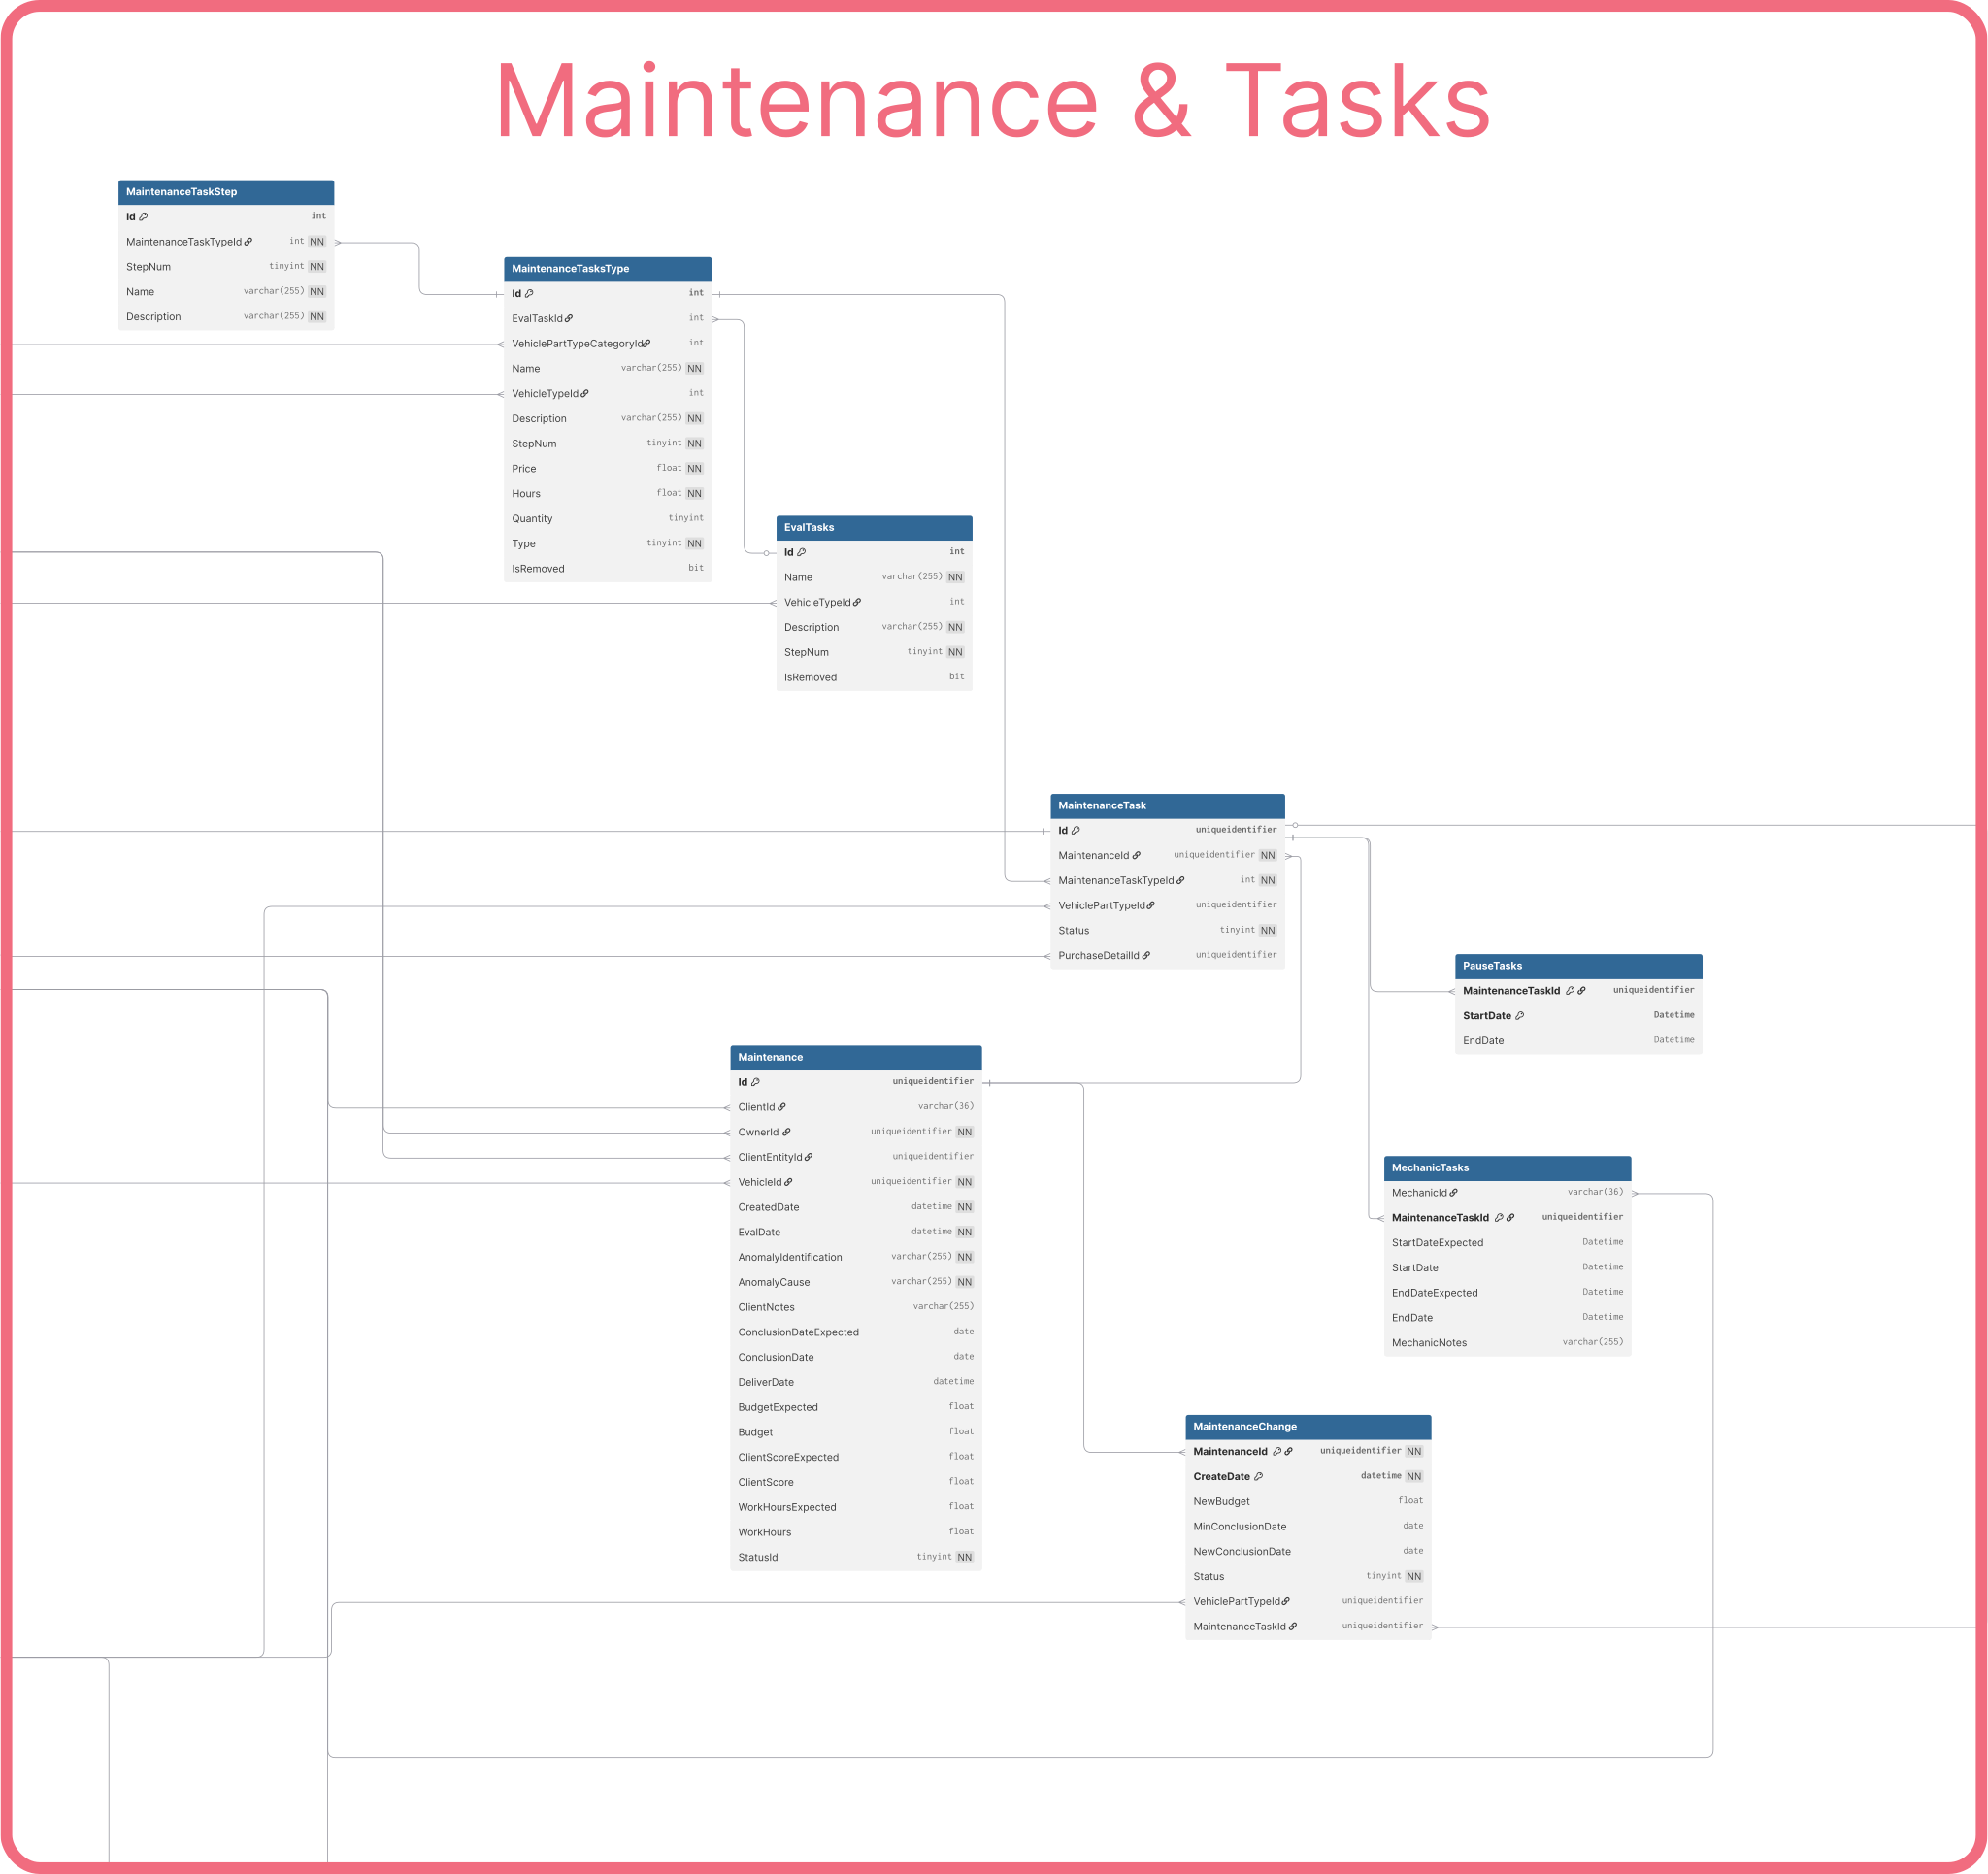
\includegraphics[width=\textwidth]{figs/dbDiagrams/Maintenance_and_Tasks}
  \label{fig:figure2}
\end{figure}

To save the information about the maintenance i created a table called the "Maintenance". This table has the following columns:
- ClientId, which is a foreign key to the AspNetUsers Table and is the table that has the information about the users of the platform.
- OwnerId, which is a foreign key to the Owners table and represents the dealership that is providing the maintenance
- VehicleId, the vehicle that is going to do the maintenance
- ClientEntityId, Optional column that connects to the Owner of a bike sharing system
- CreatedDate, that is the date of creation of the maintenance
- EvalDate, date of the evaluation date of the vehicle
- AnomalyIdentification, is a text describing the problem with the vehicle
- AnomalyCause, is a text describing the cause of the problem with the vehicle
- ClientNotes, is a text describing additional information provided by the client
- ConclusionDateExpected, is the expectedd date of the end of the maintenance agreed with the client, used to control the expectation of client for the duration of the maintenance 
- ConclusionDate, the actual date of the end of the maintenance
- DeliverDate, the date of the deliver of the vehicle to the client
- BudgetExpected, the expected budget of the maintenance agreed with the client, used to control the expectation of client for the price of the maintenance 
- Budget, the actual price of the maintenance
- ClientScoreExpected, the score of the quality of the service expected by the client
- ClientScore, the score of the quality of the service perceived by the client
- WorkHoursExpected, the number of hours expected to conclude the maintenance
- WorkHours, the number of hours to conclude the maintenance
- StatusId, the status of the maintenance. It can be WaitEvaluation, the status before the evaluation of the vehicle; waitApproval, after the evaluation of the vehicle and before the client and rececionist decide which tasks should be done, the budget of the expected budget of the maintenance and the expected conclusion date; DuringMaintenance, the status when the tasks of the maintenance are being completed; MaintenanceFinished, after all the tasks of the maintenance are completed; Delivered, when the vehicle is delivered to the client; Canceled, when the client decides to cancel the maintenance and retrieve the vehicle as it is

The maintenance is connected to the MaintenanceChange table. This table is used to save the information when a change in the maintenance occurr, like the expected conclusion date change, a task changed or the expected budget changed.
This table has the following columns:
- MaintenanceId, the identification of the maintenance which is being changed
- CreatedDate, the date of the change
- NewBudget, the new expected budget
- MinConclusionDate, the earleast date to complete the maintenance. This columns is important if, for example a part delivery is late and may only arrive on a date after the expected conclusion date.
- NewConclusionDate, the new expected conclusion date agreed with the client
- Status, the status of the maintenanceChange. It may be AskClient, when the maintenance change needs the valiation of the client; Agreed, when the client accept the changes; Refused, when the changes are refused and the maintenance keeps the same information and the previous agreement; TaskCanceled, when the client decides to cancel the task that provokes the maintenance change; MaintenanceCanceled, when the client decides to terminated the maintenance as it is.
- VehiclePartTypeId, the new part of the vehicle that from the maintenance task that is being changed
- MaintenanceTaskId, the identification of the maintenance Task that provokes the change

The maintenance is also connected with the table maintenanceTask that saves the information of the tasks from that maintenance.
This table has the following columns:
- Id, the identification of the task
- MaintenanceId, the identification of the maintenance
- MaintenanceTaskTypeId, the identification of the type of task
- VehiclePartTypeId, the identification of the type of part is used in this task
- Status, the status of the task. It may be WaitApproval, status before the approval from the client; WaitAssignment, status after the client aproval but before the workshop mananger assign it to a mechanic; Invalid, status when the client rejects the task during the maintenance agreement with the rececionist; Assigned, status when the task is assigned to a mechanic; Concluded, when the task is finished; Changed, when the mechanic notes a problem with the task and suggest a change that requires the validation from the client; WaitPart, when the part needed to complete the task is not in inventory and needs to wait for it availability to be completed.
% - PurchaseDetailId, the identification of the purchase part that is requesting the part needed to complete this task. This column allows when the purchase is complete and the parts arrive the task is notified to be able to be assigned and completed.


The maintenanceTask is connected with the table pauseTasks, that keeps tracking of the pauses of the task. 
This table has a:
- MaintenanceTaskId, that identifies the task of the maintenance
- StartDate, the start date of the pause
- EndDate, the end date of the pause

It is connected to the mechanicTasks. This table has the information of the completion of the task. It has the following columns:
- MechanicId, the identification of the mechanic
- MaintenanceTaskId, the identification of the task of the maintenance
- StatDateExpected, the date the workshop manager assigned to the mechanic starts the task
- EndDateExpected, the expected date the mechanic should end the task
- StartDate, the actual date the mechanic started the task
- EndDate, the actual date the mechanic ended the task
- MechanicNote, text left from the mechanic about the task or the vehicle


The MaintenanceTask table is also connected to the MaintenanceTaskType table. This table has the information of the type of tasks exist.
It has the following columns:
- Id, identification of the task type
- EvalTaskId, the identification of the evaluation task that can generate this type of tasks. During the evaluation period of the vehicle, if the mechanic do this evaluation task, it may add this task to the maintenance
- VehiclePartTypeCategoryId, the identification of the category of parts that this task type need to be completed
- Name, the name of the task
- Description, the description of the task
- StepNum, a integer value that represents the sequence of the tasks, for example it it has the value 2, it means it is only possible to complete this task after all tasks from stepNum 0 and 1 from this maintenance are completed
- Price, the price the client must pay to complete the task
- Hours, the number of hours estimated to complete the task
- Quantity, the number of parts is needed to complete the task
- Type, the type of maintenanceTaskType this type of maintenanceTaskType is. It may be normal, a normal task or a quality task, a task to assure the quality of the vehicle before the deliver to the client
- IsRemoved, it tells if this type of task is visible or not in the platform, this virtually seems that the task is deleted on the platform, but it can be recover if needed

The maintenanceTaskType is connected to the maintenanceTaskStep, that has the information of all the steps to complete the task.
It has the following columns:
- Id, the identification of the step
- MaintenanceTaskTypeId, the identification of the task type
- StepNum, the number of the step of the task type
- name, the name of the step
- description, the description of the step and how to complete it

The maintenanceTaskType also is connected to the EvalTasks. This table has the information about the task steps used during the evaluation of the vehicle.
It has the following columns:
- Id, the identification of the evaluation task step
- Name, the name of the evaluation task step
-VehicleTypeId, the type of vehicle that this task can be applied to
- VehiclTypeId, the identification of the type of vehicle that this task step is used on
- Description, the description of the task step
- StepNum, the step number of the task step
- IsRemoved, it tells if this type of task is visible or not in the platform


\subsection{Parts and Inventory} 


\begin{figure}[h]
  \caption{Database Parts and Inventory diagram.}
  \centering
  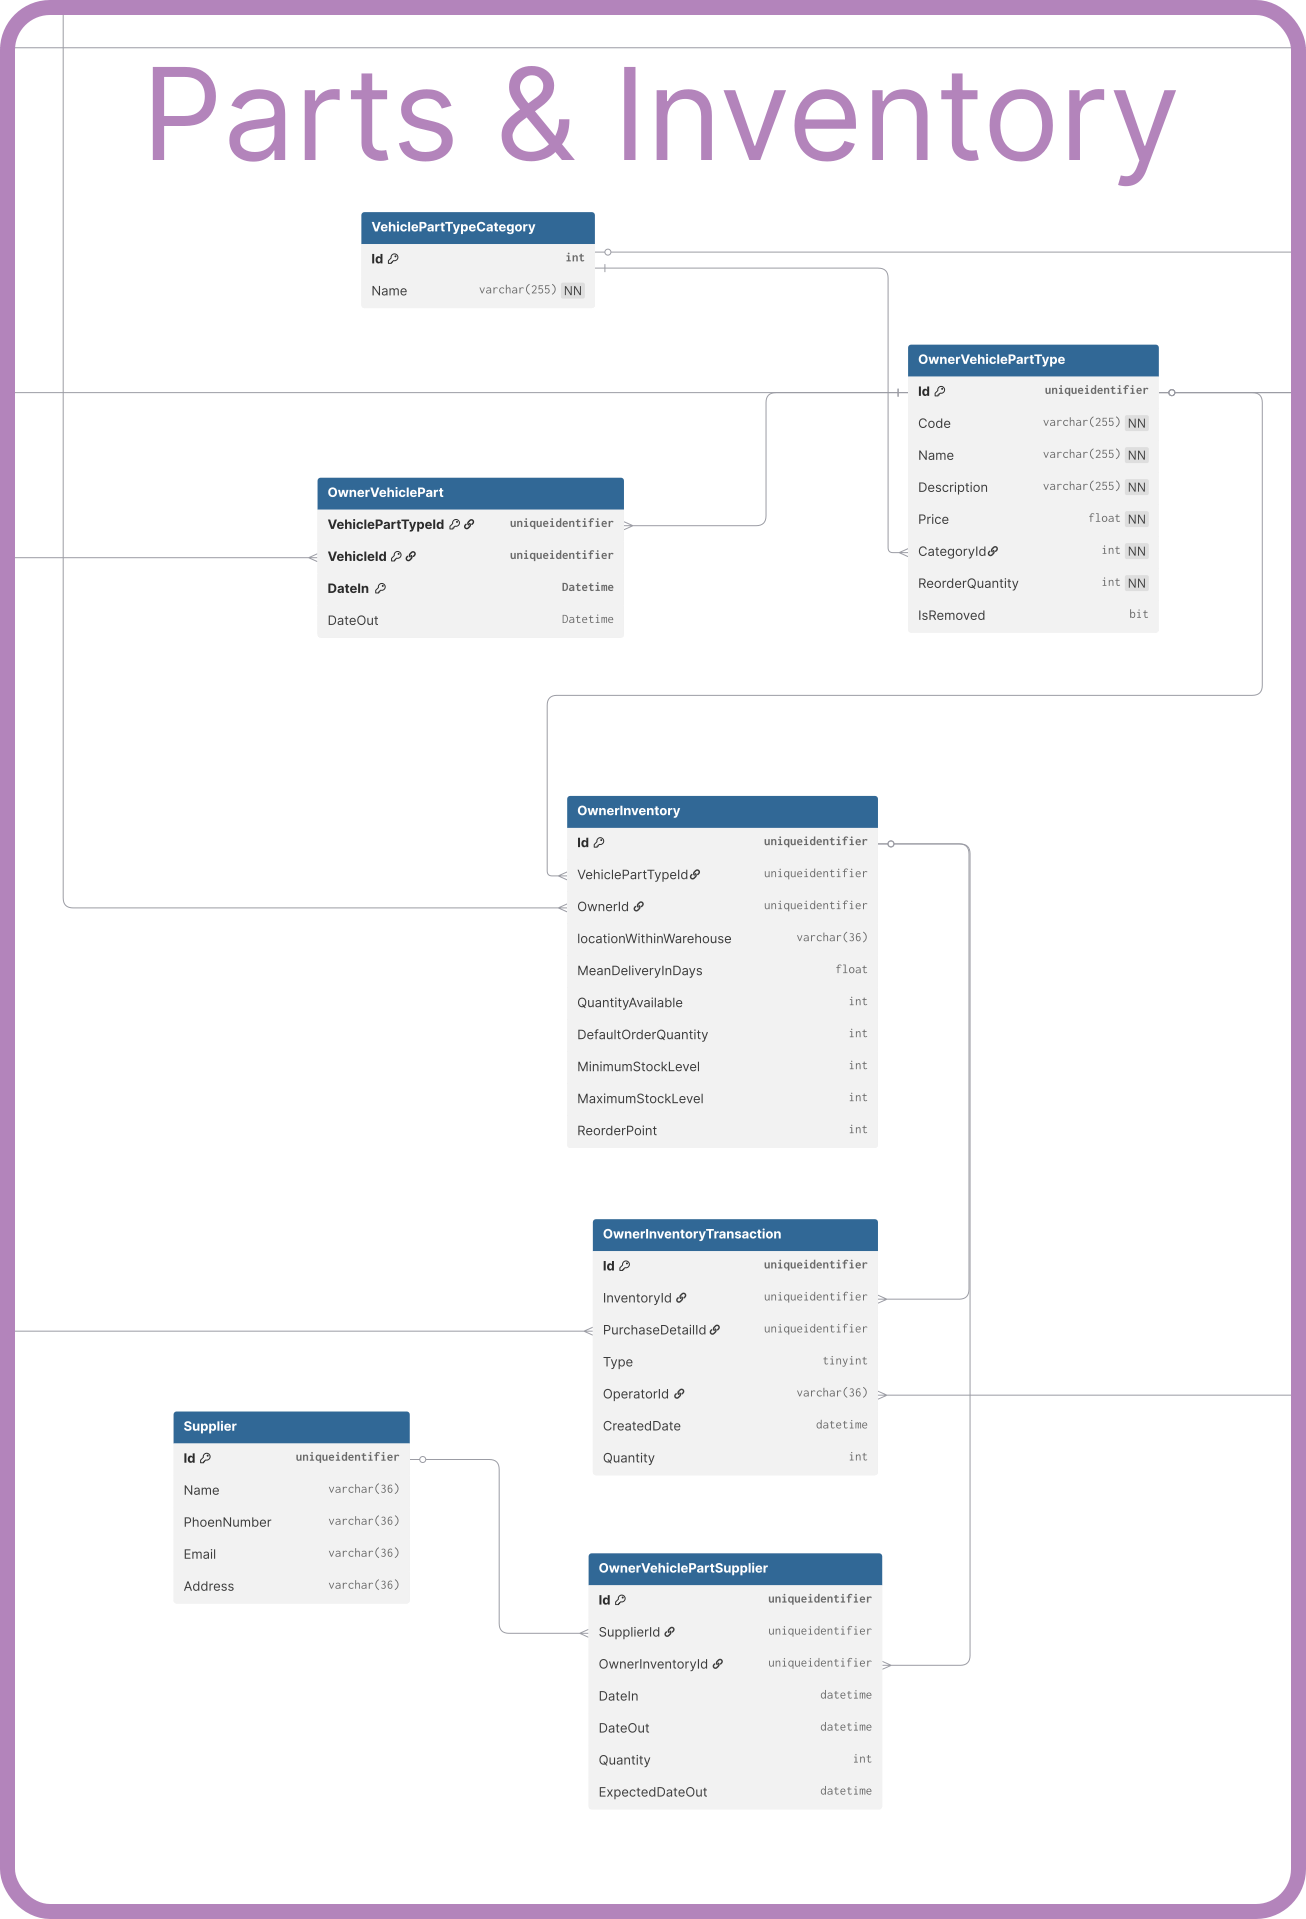
\includegraphics[width=\textwidth]{figs/dbDiagrams/Parts_and_Inventory}
  \label{fig:figure2}
\end{figure}

The inventory of the dealership is used to track the available parts on the dealership on the table OwnerInventory.
It has the following columns:
- Id, identification of the inventory
- VehiclePartTypeId, the identification of the part type of this inventory
- OwnerId, the identification of the dealership of this inventory
- LocationWithinWarehouse, is text with the code to locate the part in the warehouse of the dealership
- MeanDeliveryInDays, mean of the number of days it takes for the part to arrive at the dealership after the purchase
- QuantityAvailable, the number of parts of a specific type are available at this dealership
- DefaultOrderQuantity, the number of parts used when creating an automatic purchase for this part type when quantity on the dealership reaches a threshold
- MinimumStockLevel, the minimum number parts it the dealership should have
- MaximumStockLevel, the maximum number of parts the dealership should have
- ReorderPoint, the threshold where a purchase is created when the quantity available reaches this value

The OwnerInventory table is connected to the table OwnerInventoryTransaction, which stores the information of the sales and restock. When the quantity available changes, the action that provokes this change is saved in here.
This table has the following columns:
- Id, identification of the transaction
- InventoryId, the identification of the inventory from which occurred a sale or a restock
- PurchaseDetailId, the identification of the purchase that make the restock
- Type, if it is a restock or sale
- OperatorId, the identification of the person that provided this transaction (Warehouse Operator if it was a restock or a mechanic if it was a sale)
- CreatedDate, the date of the transaction
- Quantity, the number of parts that were added or removed from the inventory

The OwnerInventory table is also connected to the table Supplier throw the table OwnerVehiclePartSupplier.
The table supplier has the information of the suppliers of a dealership. The OwnerVehiclePartSupplier has the information of the contract between the dealership and the supplier. 
The table supplier has the following information:
- Id, the identification of the supplier
- Name, the name of the supplier
- PhoneNumber, the phonenumber of the supplier 
- Email, the email of the supplier
- Address, the address of the supplier

The OwnerVehiclePartSupplier has the following columns:
- Id, the identification of the contract
- SupplierId, the identification of the supplier
- OwnerInventoryId, the identification of the inventory of the dealership. This column identifies the dealership and the part on the contract.
- DateIn, the date that the contract starts
- DateOut, the date when the contract ended
- Quantity, the limit of parts requested in the contract
- ExpecteDateOut, the date where contract is expected to end

The OwnerInventory is also connected to the OwnerVehiclePartType that stores the type of parts exist.
This table has the following columns:
- Id, the identification of the part type
- Code, the code of the part type
- Name, the name of the part type
- Description, the description of the part type
- Price, the price of the part type
- CategoryId, the identification of category of the part type
- ReorderQuantity, the number of items per group this part must be bought with
- IsRemoved, it tells if this type of part is visible or not in the platform

This table is connected to two other tables, the VehiclePartTypeCategory and the OwnerVehiclePart.
The VehiclePartTypeCategory stores the information of the category of parts exist. 
The OwnerVehiclePart table tracks which vehicle has which parts and it already existed in the lightmobie database.
The VehiclePartTypeCategory has the following columns:
- Id, the identification of the category
- Name, the name of the category

The OwnerVehiclePart has the following columns:
- VehiclePartTypeId, the identification of the part type that the vehicle has
- VehicleId, the identification of the vehicle that has the part
- DateIn, the date when the part was inserted to the vehicle
- DateOut, the date when the part was removed from the vehicle



\subsection{Purchasing} 


\begin{figure}[h]
  \caption{Database Purchasing diagram.}
  \centering
  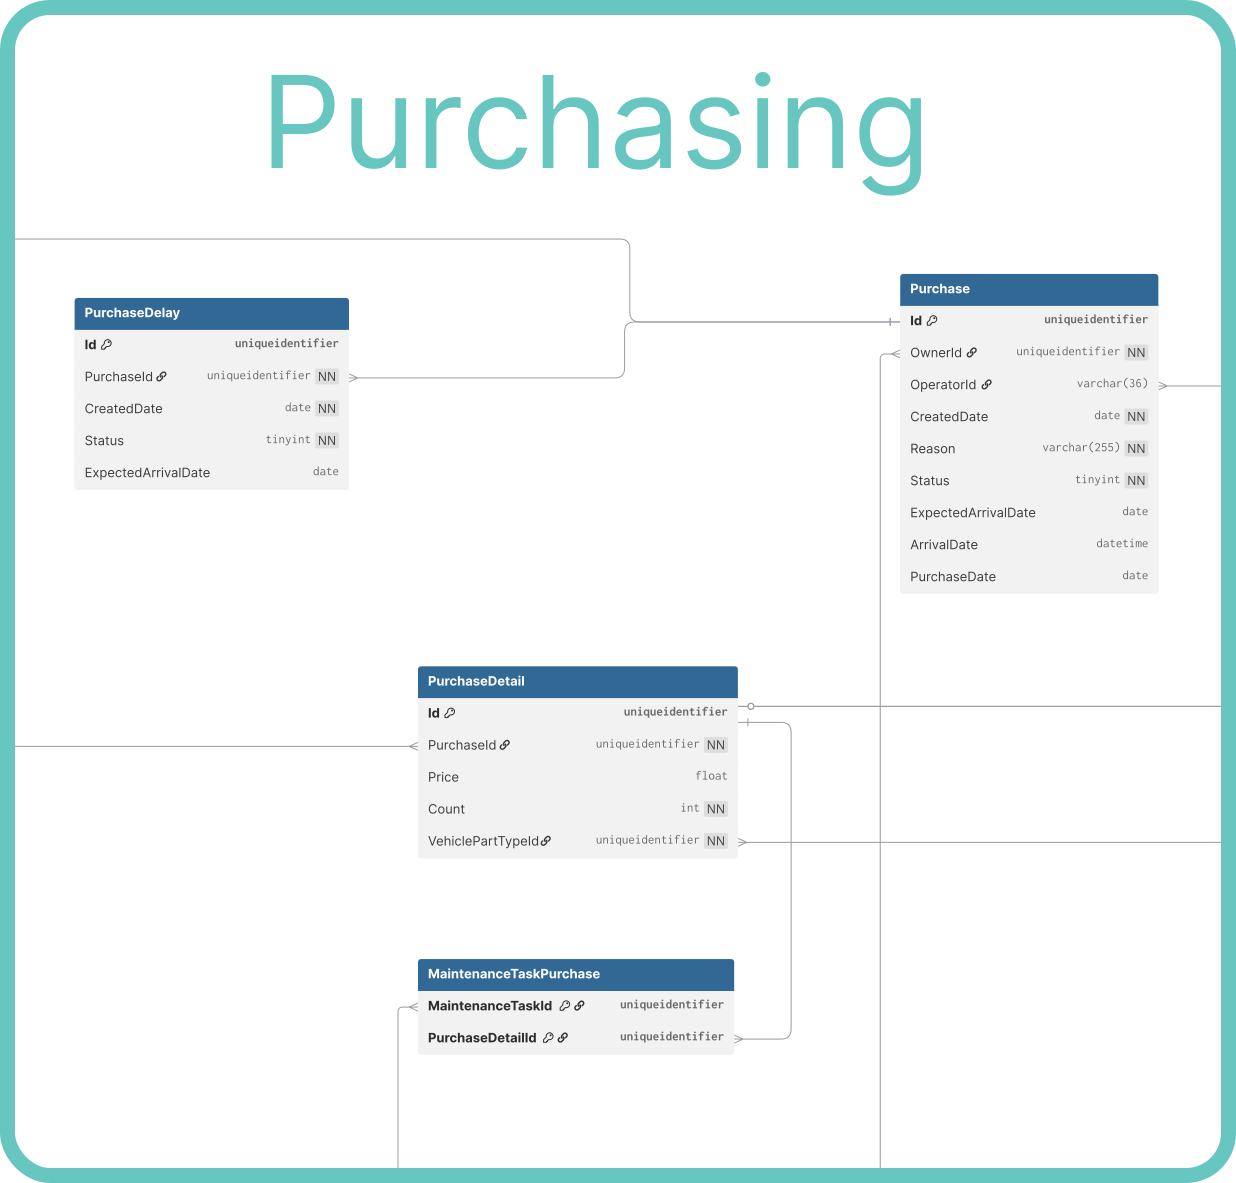
\includegraphics[width=\textwidth]{figs/dbDiagrams/Purchasing}
  \label{fig:figure2}
\end{figure}

The inventory needs purchase to restock. To this I build the table Purchase with the following columns:
- Id, the identification of the purchase
- OwnerId, the identification of the dealership that done this purchase
- OperatorId, the identification of the warehouse operator that completed the purchase
- CreatedDate, the date of the creation of the purchase
- Reason, the reason for the purchase. It is useful since the purchase needs to be verified by the workshop manager
- Status, the status of the purchase. The status may be WaitApproval, used before the purchase is approved by the workshop manager; Invalid, used when the purchase was rejected by the workshop manager; Assigned, when the purchase was approved by the workshop manager and assigned to a warehouse operator; WaitArrival, when the purchase was complete but the parts still did not arrived; Finished, after the parts arrive at the dealership
- ExpectedArrivalDate, the expected date of the arrival of the parts
- ArrivalDate, the actual date of the arrival of the parts
- PurchaseDate, the date when the purchase was done

The purchase is connected with the tables PurchaseDelay and PurchaseDetail. 
The table PurchaseDetail is used to describe the quantity of the multiple parts in a purchase.
The table PurchaseDelay is used to store the information when a purchase arrival date is delayed and the client expectation of the client due to that.
The table PurchaseDetail is also connected to the maintenanceTaskPurchase to allow a task be connected to multiple purchases due to a mistake by the mechanic and a purchase connected to multiple tasks to notify the multiple tasks that the parts have arrived.
The purchaseDetail has the following columns:
- Id, the identification of the purchaseDetail
- PurchaseId, the identification of the purchase that it is associated with
- price, the price of the part
- Count, the number of parts of this type in the purchase detail
- VehiclePartTypeId, the identification of the type of parts in the purchase detail
  
The final table, the PurchaseDelay, has the following columns:
- Id, the identification of the purchase delay
- PurchaseId, the identification of the purchase that is associated with
- CreatedDate, the date of the creation of the delay
- ExpectedArrivalDate, the new expected arrival Date


\subsection{Services} 


\begin{figure}[h]
  \caption{Database Services diagram.}
  \centering
  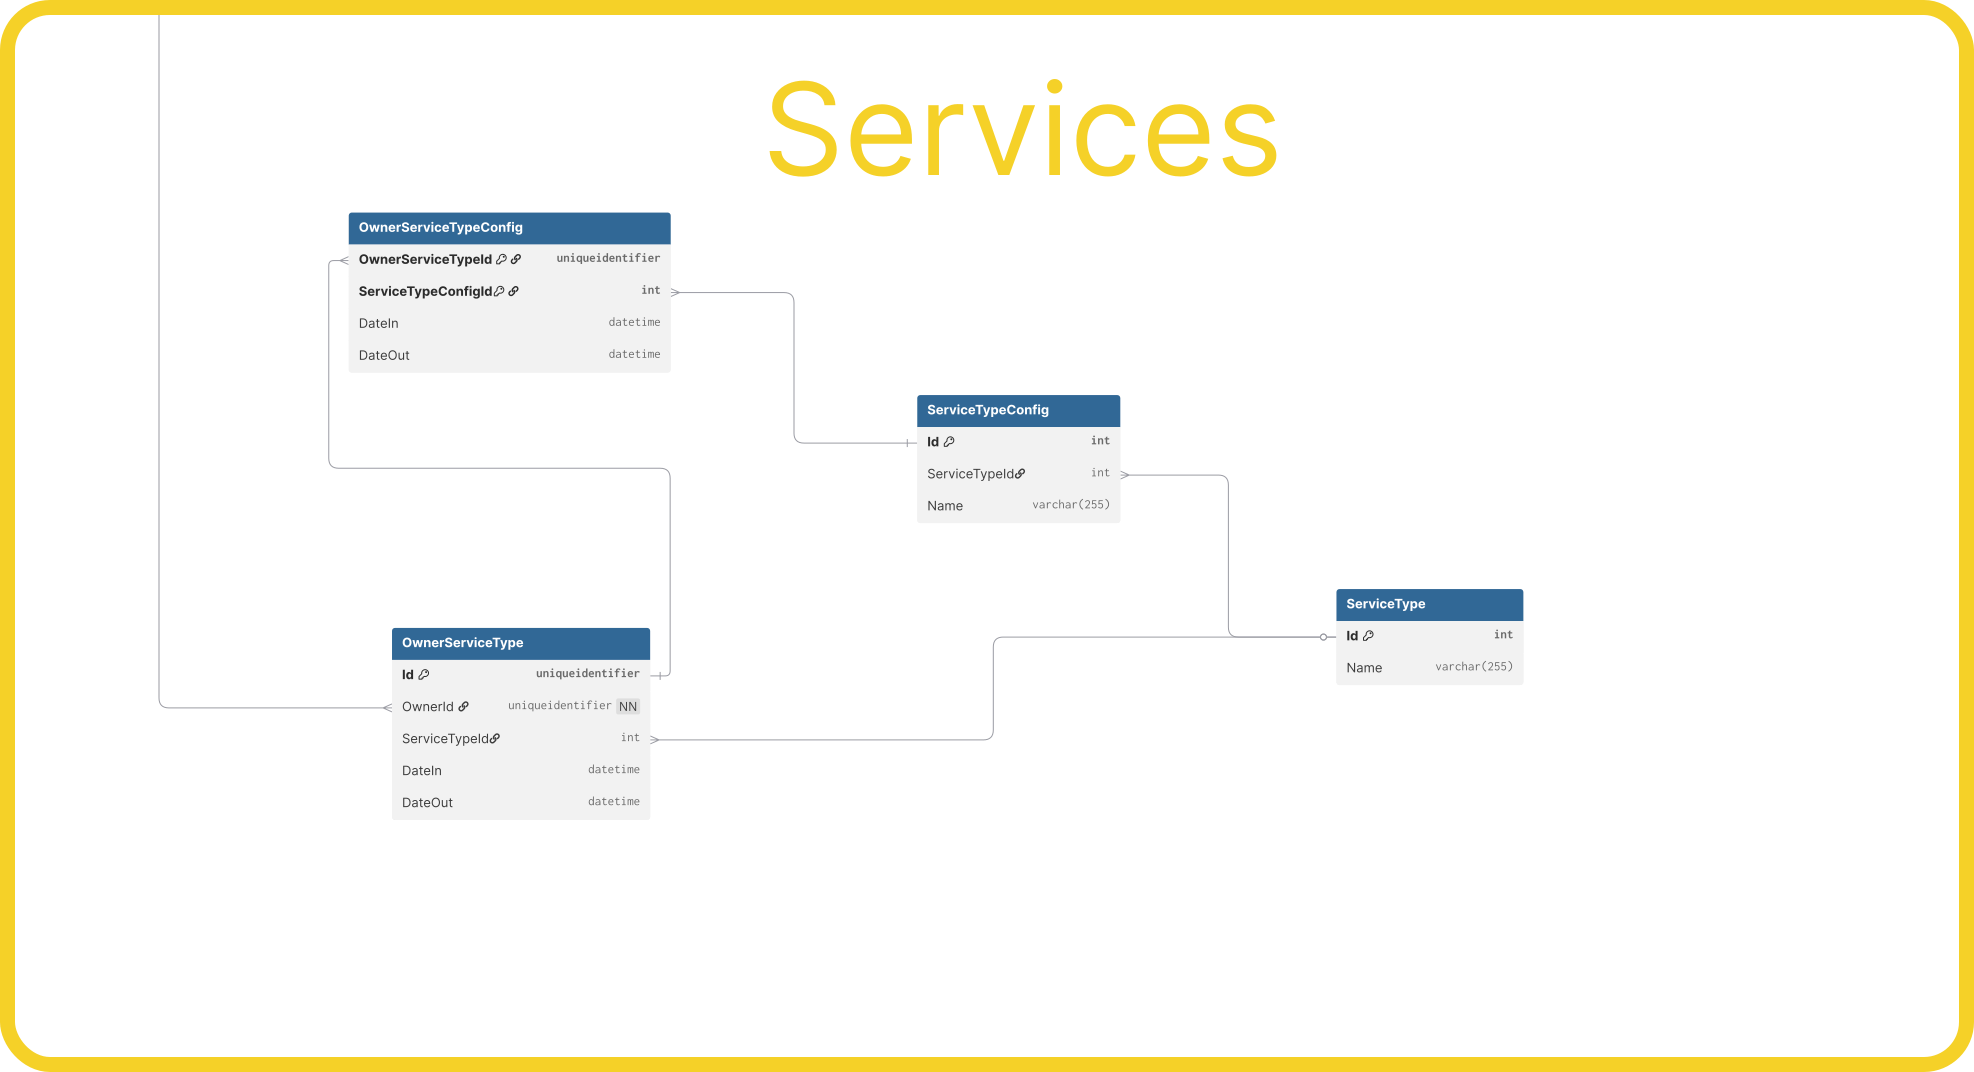
\includegraphics[width=\textwidth]{figs/dbDiagrams/Services}
  \label{fig:figure2}
\end{figure}

The services section starts with the tablke serviceType that has all type of services that exist, namely "bike sharing" and "Dealership"
This table has the following columns:
- Id, the identification of the service type
- name, the name of the service type

This table is connected with the Table Owner through the table OwnerServiceType.
This table has the info of the duration of the service to the owner.
It has the following columns:
- Id, the id of the owner service connection
- OwnerId, the identification of the owner
- ServiceType, the identification of the type of service is connected to the owner
- DateIn, the date when the service started
- DateOut, the date when the service ended

The serviceType is also connected with the table serviceTypeConfig that has the information of the various configuration of the dealership, like if does tasks division and assignment or in the evaluation it does the maintenance of the vehicle and identifies the tasks done.
It has the following columns:
- Id, the identification of the configuration
- ServiceTypeId, the identification of the service type is associated with
- Name, the name of the configuration

This table is associated with the OwnerServiceType in the table OwnerServiceTypeConfig since the dealership can chose which configuration it decides to have.
It has the following columns:
- OwnerServiceTypeId, the identification the connection of the service type and the dealership
- ServiceTypeConfigId, the identification of the configuration of the service type
- DateIn, the date when dealership start using the configuration started
- DateOut, the date when the dealership remove de configuration


\subsection{Vehicles and Owners} 


\begin{figure}[h]
  \caption{Database Vehicles and Owners diagram.}
  \centering
  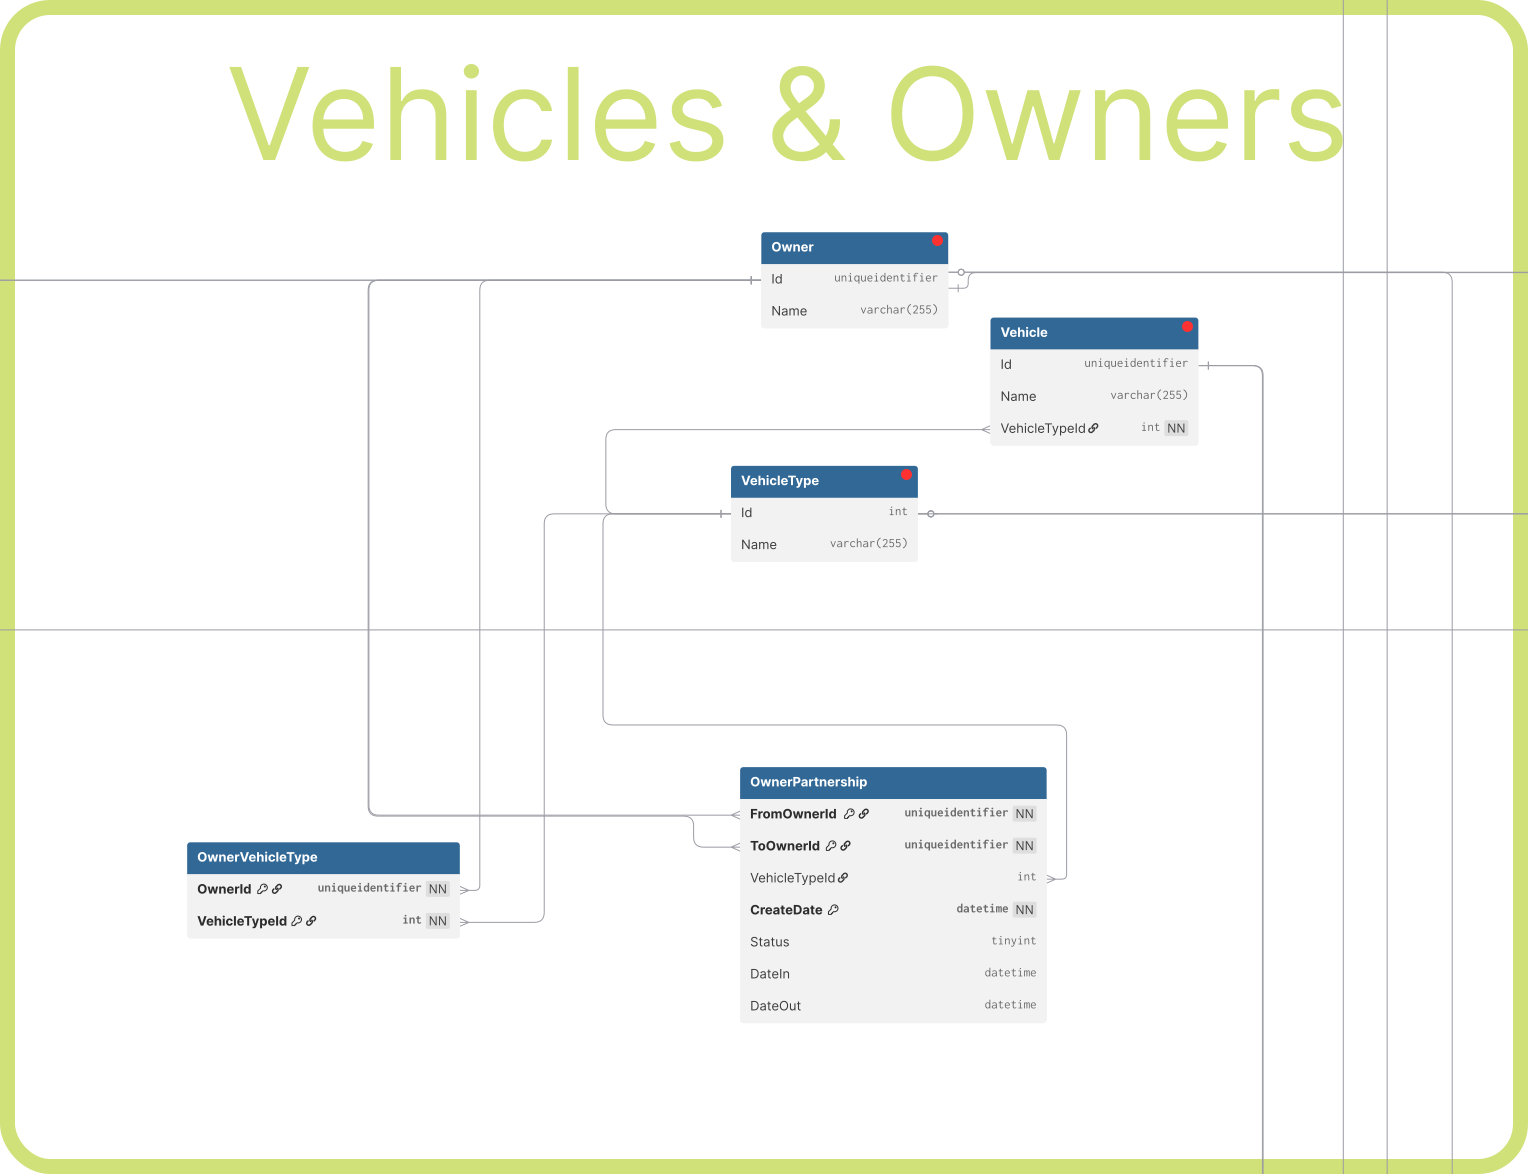
\includegraphics[width=\textwidth]{figs/dbDiagrams/Vehicles_and_Owners}
  \label{fig:figure2}
\end{figure}


This section the tables Owner, Vehicle and VehicleType already existed in the lightmobie database.
The Owner table registers the information of the dealerships and bike sharing entities.
The vehicle table registers the information of each vehicle and is connected with the vehicleType thar stores the type of vehicles, like "Eletric bikes", "convention bikes", etc.

I created the table OwnerVehicleType to allow disinguish between dealership availability to do a maintenance to specific type of vehicles. This table only has the column of connection of the two tables, owner and vehicleType.
The OwnerPartnership table is used to allow bikesharing entities to share information with dealership for it to do the maintenance. If a dealership is not connected to a bike sharing entity is not allowed to view theres vehicle information.
This table has the following columns:
- FromOwnerId, the identification of the bike sharing entity that wants to associate with the dealership
- ToOwnerId, the identification of the dealership that is requested to do maintenances to the bikesharing entity
- VehicleTypeId, the identification of the type of vehicles the bike sharing entity wants the dealership to do maintenances
- CreateDate, the date the request was created
- Status, the satus of the request, it can be Request, the request is waiting for response from the dealership; Accept, the request was accepted; Denied, the request was denied


